\documentclass{article}
\usepackage{graphicx, amsmath, amssymb, mathtools, tikz, fancyhdr, matlab-prettifier}

\usetikzlibrary{shapes, arrows, positioning}

\graphicspath{{Images/}}

\setlength{\oddsidemargin}{0in}
\setlength{\textwidth}{6.5in}
\setlength{\topmargin}{-.55in}
\setlength{\textheight}{9in}
\pagestyle{fancy}

\fancyfoot{}
\fancyhead[R]{\thepage}
\fancyhead[L]{MAE 5131}


\tikzstyle{startstop} = [rectangle, rounded corners, minimum width=3cm, minimum height = 1cm, text centered, draw = black, fill=red!30]
\tikzstyle{io} = [trapezium, trapezium left angle = 70, trapezium right angle = 110, minimum width = 3cm, minimum height = 1cm, text centered, draw=black, fill = blue!30]
\tikzstyle{process} = [rectangle, minimum width=3cm, minimum height=1cm, text centered, draw = black, fill = orange!30]
\tikzstyle{decision} = [diamond, minimum width=3cm, minimum height=1cm, text centered, draw = black, fill = green!30]
\tikzstyle{arrow} = [thick, ->, >=stealth]
\tikzstyle{connector} = [dart]

\begin{document}

\begin{center}
    {\huge Lid Driven Cavity -- Incompressible}
    \vspace{0.5cm}
    
    {\large Michael Nameika}
\end{center}

\begin{itemize}
    \item[1.]
    \begin{itemize}
        \item[(a)] For the approximations of the derivatives for the nonlinear convection terms, consider the cells above with uniform grid spacing, $h := \Delta x = \Delta y$. Then in general, for a cell-centered approach, we have
        \begin{align*}
            \frac{\partial u^2}{\partial x} &\approx \frac{(u_e)^2 - (u_w)^2}{h}\\
            \frac{\partial uv}{\partial x} &\approx \frac{u_ev_e - u_wv_w}{h}\\
            \frac{\partial uv}{\partial y} &\approx \frac{u_nv_n - u_sv_s}{h}\\
            \frac{\partial v^2}{\partial y} &\approx \frac{(v_n)^2 - (v_s)^2}{h}.
        \end{align*} 
        Using a linear interpolant to determine $u,v$ at the cell boundaries, we have 
        \begin{equation}
        \label{interps}
            \begin{aligned}
                u_e &\approx \frac{u_E + u_P}{2}, \hspace{0.4cm} u_w \approx \frac{u_P + u_W}{2}\\
                u_n &\approx \frac{u_N + u_P}{2}, \hspace{0.4cm} u_s \approx \frac{u_P + u_S}{2}\\
                v_e &\approx \frac{v_E + V_P}{2}, \hspace{0.4cm} v_w \approx \frac{v_P + v_W}{2}\\
                v_n &\approx \frac{v_N + v_P}{2}, \hspace{0.4cm} v_s \approx \frac{v_P + v_S}{2}.
            \end{aligned}
        \end{equation}
        Putting this together, we have, in general,
        \begin{align*}
            N_x &\approx \frac{1}{4h}\left((u_e)^2 - (u_w)^2 + u_nv_n - u_sv_s\right)\\
            N_y &\approx \frac{1}{4h}\left(u_ev_e - u_wv_w + (v_n)^2 - (v_s)^2\right).
        \end{align*}
        Now, on
        \begin{itemize}
            \item[(i)] the interior nodes, we can apply (\ref{interps}) so that 
            \begin{align*}
                N_x &\approx \frac{1}{4h}\left((u_E + u_P)^2 - (u_P + u_W)^2 - (u_N + u_P)(v_N + v_P) - (u_P + u_S)(v_P + v_S)\right)\\
                N_y &\approx \frac{1}{4h}\left((u_E + u_P)(v_E + v_P) - (u_P + u_W)(v_P + v_W) + (v_N + v_P)^2 - (v_P + v_S)^2\right)
            \end{align*}

            \item[(ii)] the top boundary (minus the corners), we have $u_n = 1$, $v_n = 0$. Using this with (\ref{interps}), we have
            \begin{align*}
                N_x &\approx \frac{1}{4h}\left((u_E + u_P)^2 - (u_P + u_W)^2 - (u_P + u_S)(v_P + v_S)\right)\\
                N_y &\approx \frac{1}{4h}\left((u_E + u_P)(v_E + v_P) - (u_P + u_E)(v_P + v_E) - (v_P - v_S)^2\right).
            \end{align*}

            \item[(iii)] the bottom left corner, from the boundary conditions, we have $u_w = v_w = u_s = v_s = 0$. Using this with (\ref{interps}) gives
            \begin{align*}
                N_x &\approx \frac{1}{4h}\left((u_E + u_P)^2 - (u_N + u_P)(v_N + v_P)\right)\\
                N_y &\approx \frac{1}{4h}\left((u_E + u_P)(v_E + v_P) - (v_N + v_P)^2\right)
            \end{align*}
            
        \end{itemize}


        \item[(b)] For the diffusion terms, we wish to discretize

        \begin{align*}
            L_x &= \frac{1}{Re}\left(\frac{\partial^2 u}{\partial x^2} + \frac{\partial^2 u}{\partial y^2}\right)\\
            L_y &= \frac{1}{Re}\left(\frac{\partial^2 v}{\partial x^2} + \frac{\partial^2 v}{\partial y^2}\right)
        \end{align*}
        For the cell-centered finite volume discretization, we have
        \begin{align*}
            \frac{\partial^2 u}{\partial x^2} &\approx \frac{\partial }{\partial x}\left(\frac{\partial u}{\partial x}\right)\\
            &= \frac{\left(\frac{\partial u}{\partial x}\right)_e - \left(\frac{\partial u}{\partial x}\right)_w}{h}\\
            &\approx \frac{1}{h^2} \left(u_E - u_P - u_P + u_W\right)\\
            &= \frac{u_E - 2u_P + u_W}{h^2}.
        \end{align*}
        Similarly, 
        \begin{align*}
            \frac{\partial^2 u}{\partial y^2} &\approx \frac{u_N - 2u_P + u_S}{h^2}\\
            \frac{\partial^2 v}{\partial x^2} &\approx \frac{v_E - 2v_P + v_W}{h^2}, \hspace{0.4cm} \frac{\partial v^2}{\partial y^2} \approx \frac{v_N - 2v_P + v_S}{h^2}.
        \end{align*}
        Using this on
        \begin{itemize}
            \item[(i)] the interior nodes, we have
            \begin{align*}
                L_x &\approx \frac{1}{Re}\left(\frac{u_E + u_W + u_N + u_S - 4u_P}{h^2}\right)\\
                L_y &\approx \frac{1}{Re}\left(\frac{v_E + v_W + v_N + v_S - 4v_P}{h^2}\right).
            \end{align*}

            \item[(ii)] the top boundary (minus the corners), from the boundary conditions we have $u_n = 1$, $v_n = 0$. Since our finite volume approximation only involves the nodal points, we make the assumption that the boundary conditions extend \textit{out} of the computation region. That is, we assume $u_N = 1$ and $v_N = 0$. Using this, we have
            \begin{align*}
                L_x &\approx \frac{1}{Re}\left(\frac{u_E + u_W + 1 + u_S - 4u_P}{h^2}\right)\\
                L_y &\approx \frac{1}{Re}\left(\frac{v_E + v_W + v_S - 4v_P}{h^2}\right).
            \end{align*}

            \item[(iii)] the bottom left corner. Similar to (ii), we apply the boundary conditions to $u_E = v_E = v_S = u_S = 0$
            \begin{align*}
                L_x &\approx \frac{1}{Re}\left(\frac{u_W + u_N - 4u_P}{h^2}\right)\\
                L_y &\approx \frac{1}{Re}\left(\frac{v_W + v_N - 4v_P}{h^2}\right).
            \end{align*}
        \end{itemize}

        \item[(c)] For the pressure Laplacian, we apply the same process as for diffusion terms and use Dirichlet zero boundary conditions. Doing so yields
            \begin{itemize}
            \item[(i)] for the interior nodes, 
            \begin{align*}
                \nabla^2P &\approx \frac{P_E + P_W + P_N + P_S - 4P_P}{h^2}.
            \end{align*}

            \item[(ii)] for the top boundary (minus the corners),
            \begin{align*}
                \nabla^2P &\approx \frac{P_E + P_W + P_S - 4P_P}{h^2}.
            \end{align*}

            \item[(iii)] for the bottom left corner,
            \begin{align*}
                \nabla^2P &\approx \frac{P_W + P_N - 4P_P}{h^2}.
            \end{align*}
        \end{itemize}

        \item[(d)] And finally, for the right-hand side of the pressure Poisson equation, we have
        \[R = \frac{u_e - u_w + v_n - v_s}{h}.\]
        Using (\ref{interps}), the above equation becomes
            \begin{itemize}
                \item[(i)] for the interior nodes, 
                \begin{align*}
                    R &= \frac{u_E - u_W + v_N - v_S}{h}
                \end{align*}


                \item[(ii)] for the top boundary (minus the corners), 
                \begin{align*}
                    R &= \frac{u_E - u_W - v_S}{2h}
                \end{align*}


                \item[(iii)] for the bottom left corner,
                \begin{align*}
                    R &= \frac{u_P + u_E + v_P + v_N}{2h}.
                \end{align*}
            \end{itemize}
     \end{itemize}

     %\pagebreak
     \item[2.] Flowchart \newline
     %\begin{center}
         \begin{tikzpicture}[node distance = 2cm]
            \node (start) [startstop] {Start};

            \node (pro1) [process, below of =start, align = center] {Initialize Variables: number of spatial points $N$, spatial vectors $x,y$, Reynold's number $Re$,\\ number of time steps $N_t$, initial condition for velocity field $u_0, v_0$};

            \node (pro2) [process, below of = pro1, align = center] {Define anonymous functions for the nonlinear convection terms $N_x,N_y$, diffusion terms $L_x, L_y$, and \\ right hand side of the pressure equation};

            \node (timeloop) [process, below of = pro2, align = center] {Time stepping loop};

            \node (pro3) [process, below of = timeloop, align = center] {Initialize vectors $u_{\text{new}}, v_{\text{new}}$, $u^*$, $v^*$, and $p_{\text{hold}}$. Starred variables \\ for decoupling pressure, new variables for holding next time step.\\ $p_{\text{hold}}$ for solving pressure Laplacian};

            \node (xloop) [process, below of = pro3, align = center] {Loop over $x$-indices ($i$)};

            \node (yloop) [process, below of = xloop, align = center] {Loop over $y$-indices ($j$)};

            \node (intdec) [decision, below of = yloop, align = center, yshift = -1cm] {Check: is $(x(i), y(j))$\\ an interior node?};

            \node (yesint) [process, right of = intdec, align = center, xshift = 4cm] {Compute $u^*, v^*$ at interior nodes};

            \node (boundinddec) [decision, below of = intdec, align = center, yshift = -3cm] {Is $(x(i), y(j))$ a boundary \\node but not a corner?};

            \node (boundnode) [process, left of = boundinddec, align = center, xshift = -4cm] {Compute $u^*, v^*$ \\using appropriate boundary conditions};

            \node (pageconnector) [connector, below of = boundinddec, label = right: continue on next page] {};

            \node (proCon1) [connector, below of = boundnode, yshift = -1cm] {};

            \node (proCon2) [connector, below of = yesint, yshift = -5cm] {};
            

            \draw [arrow] (start) -- (pro1);
            \draw [arrow] (pro1) -- (pro2);
            \draw [arrow] (pro2) -- (timeloop);
            \draw [arrow] (timeloop) -- (pro3);
            \draw [arrow] (pro3) --(xloop);
            \draw [arrow] (xloop) -- (yloop);
            \draw [arrow] (yloop) -- (intdec);
            \draw [arrow] (intdec) -- (yesint);
            \draw [arrow] (intdec) -- (boundinddec);
            \draw [arrow] (boundinddec) -- (boundnode);
            \draw [arrow] (yesint) -- (proCon2);
            \draw [arrow] (boundnode) -- (proCon1);
         \end{tikzpicture}
        
         \begin{tikzpicture}
             \node (newcon) [connector, label = right:continued] {};
             
             \node (cornerdec) [decision, align = center, below of = newcon, yshift = -1.5cm] {Is $(x(i), x(j))$ a \\
             corner node?};

             \node (corncomp) [process, align = center, right of = cornerdec, xshift = 4cm] {Compute $u^*, v^*$ using \\ appropriate boundary conditions};

            \node (pupdate) [process, align = center, below of = cornerdec, yshift = -2cm] {Update $pHold$ using $R$};

            \node (plaplace) [process, align = center, below of = pupdate, yshift = -1cm] {Solve pressure laplacian};

            \node (pgradient) [process, align = center, below of = plaplace, yshift = -1cm] {Compute pressure gradient, update $u_{\text{new}}, v_{\text{new}}$};

            \node (endloops) [process, align = center, below of = pgradient, yshift = -1cm] {End time stepping loop, $x$ index loop, $y$ index loop};

            \node (plot) [process, align = center, below of = endloops, yshift = -1cm] {Plot velocity field, pressure contours, streamlines};

            \node (end) [startstop, align = center, below of = plot, yshift = -1cm] {End};


            \draw [arrow] (corncomp) -- (pupdate);

            \draw [arrow] (newcon) -- (cornerdec);
            \draw [arrow] (cornerdec) -- (corncomp);
            \draw [arrow] (cornerdec) -- (pupdate);
            \draw [arrow] (pupdate) -- (plaplace);
            \draw [arrow] (plaplace) -- (pgradient);
            \draw [arrow] (pgradient) -- (endloops);
            \draw [arrow] (endloops) -- (plot);
            \draw [arrow] (plot) -- (end);
         \end{tikzpicture}
         
    \pagebreak
     \item[3.] Implementing the above Finite Volume approach for this problem, we find the following results for $N = 50,100,200$ at the nondimensional time $t = 20$:
    \begin{center}
        \includegraphics[scale = 0.13]{N_50.png}
        \includegraphics[scale = 0.13]{N_100.png}
        \includegraphics[scale = 0.18]{N_200.png}
    \end{center}


     Note that the pressure is lowest in the upper left corner and highest at the upper right corner. This intuitively makes sense since the upper left corner has a most amount of flow away from it and the upper right hand corner has the highest flow towards it. Note also that there is a cyclic region near the center, with small amounts of rotation throughout the rest of the cavity, as is displayed by the streamlines. Further notice that the streamline near the rotational center moves into a more stable orbit for a larger number of spatial points.



     \pagebreak
     \item[4.] Code:
    \begin{center}
        \begin{lstlisting}[style = Matlab-editor]
            %finite volume NS implementation
clear all; close all;

%number of spatial points
Nx = 200;
Ny = Nx;

%spatial grid spacing
h = 1/(Nx-2);
% h = 1/(Nx - 1);

%initial and final times
t0 = 0;
tEnd = 20;

%time step size
dt = 0.01/8;

%number of time steps
Nt = (tEnd - t0)/dt;

%Reynold's number
Re = 200;

%spatial coordinates
x = [0 h/2:h:1-h/2 1];
% x = linspace(0,1,Nx);
y = x;

%meshgrid plots for x and y for plotting purposes
[Xplot, Yplot] = meshgrid(x,y);

%initial conditions for velocity field
u0 = zeros(Nx,Ny);
u0(:,end) = 1;

v0 = zeros(Nx,Ny);


%Laplacian operator for solving pressure poisson equation
onesVec = ones(Nx,1);

%second derivative matrix
D2 = 1/h^2*spdiags([onesVec -2*onesVec onesVec], [-1 0 1], Nx, Ny);

I = speye(Nx,Nx);

%5 point laplacian matrix
Lop = kron(D2,I) + kron(I,D2);

%nonlinear convection terms
N_x = @(ue,uw,un,us,ve,vw,vn,vs) 1/h*( ue^2 - uw^2 + un*vn - us*vs );
N_y = @(ue,uw,un,us,ve,vw,vn,vs) 1/h*( ue*ve - uw*vw + vn^2 - vs^2 );

%diffusion terms
%use ghost cells for boundary conditions
L_x = @(uP,uE,uW,uN,uS) 1/(Re*h^2)*( uN + uW + uS + uE - 4*uP );
L_y = @(vP,vE,vW,vN,vS) 1/(Re*h^2)*( vN + vW + vS + vE - 4*vP );

%RHS of pressure equation
R = @(ue,uw,un,us,ve,vw,vn,vs) 1/h*( ue - uw + vn - vs );


%time stepping
for k = 1:Nt
    %initialize the starred variablesx
    unew = zeros(Nx,Ny);
    vnew = zeros(Nx,Ny);

    ustar = zeros(Nx,Ny);
    vstar = zeros(Nx,Ny);

    pHold = zeros(Nx,Ny);
    
    for i = 1:Nx
        for j = 1:Ny
            
            %interior nodes
            if (i > 1 && i < Nx && j > 1 && j < Ny)

                %interpolate nodes 
                ue = (u0(i+1,j) + u0(i,j))/2;
                uw = (u0(i-1,j) + u0(i,j))/2;
                un = (u0(i,j+1) + u0(i,j))/2;
                us = (u0(i,j-1) + u0(i,j))/2;

                ve = (v0(i+1,j) + v0(i,j))/2;
                vw = (v0(i-1,j) + v0(i,j))/2;
                vn = (v0(i,j+1) + v0(i,j))/2;
                vs = (v0(i,j-1) + v0(i,j))/2;

                
                N1 = N_x(ue, uw, un, us, ve, vw, vn, vs);
                N2 = N_y(ue, uw, un, us, ve, vw, vn, vs);

                L1 = L_x(u0(i,j), u0(i+1,j), u0(i-1,j), u0(i,j+1), u0(i,j-1));
                L2 = L_y(v0(i,j), v0(i+1,j), v0(i-1,j), v0(i,j+1), v0(i,j-1));

                R1 = R(ue, uw, un, us, ve, vw, vn, vs);

                ustar(i,j) = u0(i,j) - dt*N1 + dt*L1;
                vstar(i,j) = v0(i,j) - dt*N2 + dt*L2;
                
            %Bottom boundary NO CORNERS
            elseif (i > 1 && i < Nx && j == 1)
                ue = (u0(i+1,j) + u0(i,j))/2;
                uw = (u0(i-1,j) + u0(i,j))/2;
                un = (u0(i,j+1) + u0(i,j))/2;
                us = 0;

                ve = (v0(i+1,j) + v0(i,j))/2;
                vw = (v0(i-1,j) + v0(i,j))/2;
                vn = (v0(i,j+1) + v0(i,j))/2;
                vs = 0;

                
                N1 = N_x(ue, uw, un, us, ve, vw, vn, vs);
                N2 = N_y(ue, uw, un, us, ve, vw, vn, vs);

                L1 = L_x(u0(i,j), u0(i+1,j), u0(i-1,j), u0(i,j+1), 0);
                L2 = L_y(v0(i,j), v0(i+1,j), v0(i-1,j), v0(i,j+1), 0);

                R1 = R(ue, uw, un, us, ve, vw, vn, vs);

                ustar(i,j) = u0(i,j) - dt*N1 + dt*L1;
                vstar(i,j) = v0(i,j) - dt*N2 + dt*L2;

            %top boundary NO CORNERS
            elseif (i > 1 && i < Nx && j == Ny)
                ue = (u0(i+1,j) + u0(i,j))/2;
                uw = (u0(i-1,j) + u0(i,j))/2;
                un = 1;
                us = (u0(i,j-1) + u0(i,j))/2;

                ve = (v0(i+1,j) + v0(i,j))/2;
                vw = (v0(i-1,j) + v0(i,j))/2;
                vn = 0;
                vs = (v0(i,j-1) + v0(i,j))/2;

                
                N1 = N_x(ue, uw, un, us, ve, vw, vn, vs);
                N2 = N_y(ue, uw, un, us, ve, vw, vn, vs);

                L1 = L_x(u0(i,j), u0(i+1,j), u0(i-1,j), 1, u0(i,j-1));
                L2 = L_y(v0(i,j), v0(i+1,j), v0(i-1,j), 0, v0(i,j-1));

                R1 = R(ue, uw, un, us, ve, vw, vn, vs);

                ustar(i,j) = u0(i,j) - dt*N1 + dt*L1;
                vstar(i,j) = v0(i,j) - dt*N2 + dt*L2;
            
            %left boundary NO CORNERS
            elseif (j > 1 && j < Ny && i == 1)
                ue = (u0(i+1,j) + u0(i,j))/2;
                uw = 0;
                un = (u0(i,j+1) + u0(i,j))/2;
                us = (u0(i,j-1) + u0(i,j))/2;

                ve = (v0(i+1,j) + v0(i,j))/2;
                vw = 0;
                vn = (v0(i,j+1) + v0(i,j))/2;
                vs = (v0(i,j-1) + v0(i,j))/2;

                
                N1 = N_x(ue, uw, un, us, ve, vw, vn, vs);
                N2 = N_y(ue, uw, un, us, ve, vw, vn, vs);

                L1 = L_x(u0(i,j), u0(i+1,j), 0, u0(i,j+1), u0(i,j-1));
                L2 = L_y(v0(i,j), v0(i+1,j), 0, v0(i,j+1), v0(i,j-1));

                R1 = R(ue, uw, un, us, ve, vw, vn, vs);

                ustar(i,j) = u0(i,j) - dt*N1 + dt*L1;
                vstar(i,j) = v0(i,j) - dt*N2 + dt*L2;


            %right boundary NO CORNERS
            elseif (j > 1 && j < Ny && i == Nx)
                ue = 0;
                uw = (u0(i-1,j) + u0(i,j))/2;
                un = (u0(i,j+1) + u0(i,j))/2;
                us = (u0(i,j-1) + u0(i,j))/2;

                ve = 0;
                vw = (v0(i-1,j) + v0(i,j))/2;
                vn = (v0(i,j+1) + v0(i,j))/2;
                vs = (v0(i,j-1) + v0(i,j))/2;

                
                N1 = N_x(ue, uw, un, us, ve, vw, vn, vs);
                N2 = N_y(ue, uw, un, us, ve, vw, vn, vs);

                L1 = L_x(u0(i,j), 0, u0(i-1,j), u0(i,j+1), u0(i,j-1));
                L2 = L_y(v0(i,j), 0, v0(i-1,j), v0(i,j+1), v0(i,j-1));

                R1 = R(ue, uw, un, us, ve, vw, vn, vs);

                ustar(i,j) = u0(i,j) - dt*N1 + dt*L1;
                vstar(i,j) = v0(i,j) - dt*N2 + dt*L2;

            %bottom left corner
            elseif (i == 1 && j == 1)
                ue = (u0(i+1,j) + u0(i,j))/2;
                uw = 0;
                un = (u0(i,j+1) + u0(i,j))/2;
                us = 0;

                ve = (v0(i+1,j) + v0(i,j))/2;
                vw = 0;
                vn = (v0(i,j+1) + v0(i,j))/2;
                vs = 0;

                
                N1 = N_x(ue, uw, un, us, ve, vw, vn, vs);
                N2 = N_y(ue, uw, un, us, ve, vw, vn, vs);

                L1 = L_x(u0(i,j), u0(i+1,j), 0, u0(i,j+1), 0);
                L2 = L_y(v0(i,j), v0(i+1,j), 0, v0(i,j+1), 0);

                R1 = R(ue, uw, un, us, ve, vw, vn, vs);

                ustar(i,j) = u0(i,j) - dt*N1 + dt*L1;
                vstar(i,j) = v0(i,j) - dt*N2 + dt*L2;

            %top left corner
            elseif (i == 1 && j == Ny)
                ue = (u0(i+1,j) + u0(i,j))/2;
                uw = 0;
                un = 1;
                us = (u0(i,j-1) + u0(i,j))/2;

                ve = (v0(i+1,j) + v0(i,j))/2;
                vw = 0;
                vn = 0;
                vs = (v0(i,j-1) + v0(i,j))/2;

                
                N1 = N_x(ue, uw, un, us, ve, vw, vn, vs);
                N2 = N_y(ue, uw, un, us, ve, vw, vn, vs);

                L1 = L_x(u0(i,j), u0(i+1,j), 0, 1, u0(i,j-1));
                L2 = L_y(v0(i,j), v0(i+1,j), 0, 0, v0(i,j-1));

                R1 = R(ue, uw, un, us, ve, vw, vn, vs);

                ustar(i,j) = u0(i,j) - dt*N1 + dt*L1;
                vstar(i,j) = v0(i,j) - dt*N2 + dt*L2;

            %bottom right corner
            elseif (i == Nx && j == 1)
                ue = 0;
                uw = (u0(i-1,j) + u0(i,j))/2;
                un = (u0(i,j+1) + u0(i,j))/2;
                us = 0;

                ve = 0;
                vw = (v0(i-1,j) + v0(i,j))/2;
                vn = (v0(i,j+1) + v0(i,j))/2;
                vs = 0;

                
                N1 = N_x(ue, uw, un, us, ve, vw, vn, vs);
                N2 = N_y(ue, uw, un, us, ve, vw, vn, vs);

                L1 = L_x(u0(i,j), 0, u0(i-1,j), u0(i,j+1), 0);
                L2 = L_y(v0(i,j), 0, v0(i-1,j), v0(i,j+1), 0);

                R1 = R(ue, uw, un, us, ve, vw, vn, vs);

                ustar(i,j) = u0(i,j) - dt*N1 + dt*L1;
                vstar(i,j) = v0(i,j) - dt*N2 + dt*L2;

            %top right corner
            elseif (i == Nx && j == Ny)
                ue = 0;
                uw = (u0(i-1,j) + u0(i,j))/2;
                un = 1;
                us = (u0(i,j-1) + u0(i,j))/2;

                ve = 0;
                vw = (v0(i-1,j) + v0(i,j))/2;
                vn = 0;
                vs = (v0(i,j-1) + v0(i,j))/2;

                
                N1 = N_x(ue, uw, un, us, ve, vw, vn, vs);
                N2 = N_y(ue, uw, un, us, ve, vw, vn, vs);

                L1 = L_x(u0(i,j), 0, u0(i-1,j), 1, u0(i,j-1));
                L2 = L_y(v0(i,j), 0, v0(i-1,j), 0, v0(i,j-1));

                R1 = R(ue, uw, un, us, ve, vw, vn, vs);

                ustar(i,j) = u0(i,j) - dt*N1 + dt*L1;
                vstar(i,j) = v0(i,j) - dt*N2 + dt*L2;
            end



             %solve for the pressure
            pHold(i,j) = 1/dt*R(ue,uw,un,us,ve,vw,vn,vs);
           
        end %end y indexing for loop
    end %end x indexing for loop


    pHold = reshape(pHold, Nx*Ny, 1);

    pHold = Lop\pHold;

    pHold = reshape(pHold, Nx,Ny);

    for i = 2:Nx-1
        for j = 2:Ny-1
            Px = 1/(2*h)*( pHold(i+1,j) - pHold(i-1,j) );
            Py = 1/(2*h)*( pHold(i,j+1) - pHold(i,j-1) );

            %update velocity field
            unew(i,j) = ustar(i,j) - dt*Px;
            vnew(i,j) = vstar(i,j) - dt*Py;

        end
    end

    %update velocity values
    u0 = unew;
    u0(:,end) = 1;

    v0 = vnew;

    %display progress of number of time steps
    prog = k/Nt

end %end time stepping loop


%fine grid
NFine = Nx^2/4;
xFine = linspace(0,1,NFine);
yFine = xFine;

XFine = Xplot;
YFine = Yplot;
pFine = pHold;
% [XFine, YFine] = meshgrid(xFine, yFine);
% pFine = interp2(Xplot,Yplot, pHold, XFine, YFine, 'spline');


contourf(XFine, YFine, pFine', -1:0.01:1, 'LineStyle', 'none')
hold on
qspace = 10;

quiver(Xplot(1:qspace:end,1:qspace:end), Yplot(1:qspace:end,1:qspace:end), u0(1:qspace:end,1:qspace:end)',v0(1:qspace:end,1:qspace:end)', 1, 'k-', 'linewidth', 0.5)
cb = colorbar();
colormap('Turbo')
% hold off

axis([0 1 0 1])
xlabel('$x$', 'fontsize', 45, 'interpreter', 'latex')
ylabel('$y$', 'fontsize', 45, 'interpreter', 'latex')
ylabel(cb, 'Pressure $P$', 'fontsize', 45, 'interpreter', 'latex')

strmln1 = stream2(Xplot,Yplot, u0',v0', 0.7755,0.7755);
strmln2 = stream2(Xplot,Yplot, u0', v0', 0.883, 0.1378);
strmln3 = stream2(Xplot,Yplot, u0', v0', 0.7602, 0.413);
strmln4 = stream2(Xplot,Yplot, u0', v0', 0.6786, 0.7092);

strmPts = 2000;

strmDbl1 = strmln1{1};
strmDbl2 = strmln2{1};
strmDbl3 = strmln3{1};
strmDbl4 = strmln4{1};

plot(strmDbl1(1:strmPts,1), strmDbl1(1:strmPts,2), 'k-', 'linewidth', 0.8)
plot(strmDbl2(:,1), strmDbl2(:,2), 'k-', 'linewidth', 0.8)
% plot(strmDbl3(:,1), strmDbl3(:,2), 'k-', 'linewidth', 0.8)
% plot(strmDbl4(:,1), strmDbl4(:,2), 'k-', 'linewidth', 0.8)

hold off
title("Velocity field for lid driven cavity ($N = $ " + Nx + ", $\Delta t = $ " + dt + ")", 'fontsize', 25, 'interpreter', 'latex')
        \end{lstlisting}
    \end{center}
     
\end{itemize}

\end{document}
